\section{Compiling}
\subsection{Introduction}
A full computing environment is not complete without a compiler that generates the machine code from some human readable programming language. One could argue that Brainf*ck \emph{is} the programming language, but to say it's human readable is a bit of a stretch. The aim of this chapter is to describe the fundamentals behind the Acus library, which exposes a set of elementary assembly-like instructions (like arithmetic operations, conditional expressions and jumps) that are compiled into BF. It is meant as a compiler back-end that can be used to build a fully fledged programming language on top of. Since BF is lacking arbitrary code-jumps or memory accesses, multiple abstractions had to be built on top of the raw BF tape-cells in order for jumps and random memory access to be simulated at runtime. This allows high-level abstractions like function-calls and pointer-arithmetic to be implemented in terms of primitive BF instructions.

\subsection{Program Structure}
In the Acus model, a program consists of a series of basic blocks, sequences of code that are always executed in order, and jumps between those blocks. Each basic block is compiled into its corresponding BF instructions and placed in a BF loop-pair (i.e.~ between\texttt{[} and \texttt{]}). The complete sequence of blocks is enclosed in a main-loop, conditional on the value in a special BF-cell, the \emph{Run}-cell, which can be reset by any block when the program should be terminated:

\begin{center}
  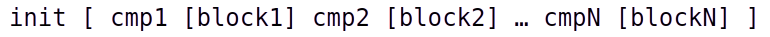
\includegraphics[width=0.8\textwidth]{img/program_structure}
\end{center}


Each block in the main loop is preambled by some code that compares the value of another predefined cell, the \emph{TargetBlock}-cell, to the block-index of the code-block. Only when this cell contains the exact index of the block \emph{and} the \emph{Run}-cell is still nonzero, is the loop entered and its code executed. Therefore, each block should at some point set the index of next block to be executed to keep the program going. This approach basically implements a state-machine that can be expressed in pseudo-code as shown in Listing \ref{lst:acusprogram}.

\begin{lstfloat}[H]
  \begin{lstlisting}[style=pseudocode]
    blocks = [block1, block2, ..., blockN]

    Run = 1
    TargetBlock = 1

    while Run:
      for index = 1:N
        if Run AND TargetBlock == index:
          execute blocks[index]
  \end{lstlisting}
  \caption{Pseudocode of an Acus-generated program.}
  \label{lst:acusprogram}
\end{lstfloat}

\subsubsection*{Example: Fibonacci}
To illustrate how a program is divided into basic blocks, a simple fibonacci number generator is shown in Figure \ref{fig:fibexample}. It consists of three functions, each of which contains multiple basic blocks. The block-ID's are shown in square brackets at the start of each block. Blocks end at control-boundaries, i.e.~ places in the code where potential jumps take place or explicitly at predefined labels.

The program starts execution in block 10, which is set as the entry-point by the initialization code (it was set to ID 1 in the pseudocode of Listing \ref{lst:acusprogram}). A function-call is immediately encountered, ending the current block. After initializing a new stack-frame (this will be covered later, in Section \ref{sec:noideayet}), the \emph{TargetBlock} is set to block 1. This will cause control flow to skip over block 11 and loop back to block 1, which will then be entered. When control hits the conditional statement of block 3, either block 4 or 5 will be set as the next target-block, depending on the result of evaluating \texttt{i<n}. In this case, both the \texttt{if}- and \texttt{else} body contain only a single block that immediately terminates in a jump. When control eventually reaches the end of \texttt{main}, the \emph{Run}-cell is set to zero, causing flow to exit the main loop and terminate the program.

\begin{figure}[H]
  \centering
  \begin{subfigure}{0.4\linewidth}
    \centering
    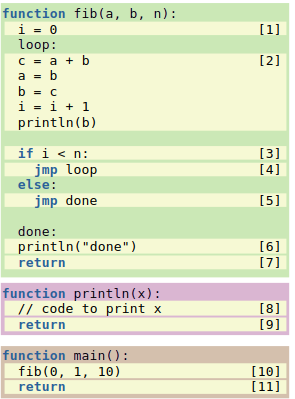
\includegraphics[height=10cm]{img/fib_blocks}
    \caption{Fibonacci program}
    \label{fig:fibblocks}
  \end{subfigure}
  \hspace{1cm}
  \begin{subfigure}{0.4\linewidth}
    \centering
    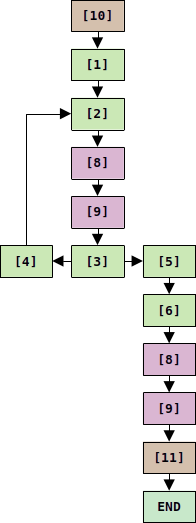
\includegraphics[height=10cm]{img/fib_flow}
    \caption{Control flow}
    \label{fig:fibflow}
  \end{subfigure}
  \caption{Figure (a) shows a simple fibonacci program (unspecified syntax) and how that program is split into blocks. Figure (b) shows how control flows from one block to another.}
  \label{fig:fibexample}
\end{figure}

\subsection{Tape Abstractions}
The data-tape is considered a stack, where each function owns a stack-frame. Each frame contains a return-slot (if the function returns a value), argument-slots (if the function takes arguments) and local data (variables and temporaries used in the function). A slot is a series of (logical) cells that variables of different data-types used by the function. The size of the slot depends on the number of cells required to represent the type of the variable. Instead of using single BF-cells to compose slots, logical cells or macro-cells are used. Each macro-cell contains 9 actual BF-cells, referred to as \emph{fields} from now on, each of which serves a different purpose. Central to the macro-cells are the two value-fields that hold the actual value of the logical cell. By having two value fields, we allow for 16-bit datatypes to be implemented within the same logical-cell, rather than having to allocate two macro-cells for a single 16-bit variable. The other fields hold temporary data or metadata required to perform higher level functions like arithmetic, flow control and dynamic pointer movement. When the compiler needs to generate code that moves the BF-pointer to location known only at runtime (for example when dereferencing pointers or accessing array elements by a dynamic index), these fields can hold temporary values or metadata necessary to perform the move. Other non-value fields include temporary scratch-pads (heavily used when performing arithmetic operations), payload-fields (used to transport data to locations known at runtime) and a flag cell that is dedicated to the evaluation of loop-conditions. Having all these fields near each other on the BF-tape has the nice consequence of BF-algorithms being relatively short due to tight pointer-move-sequences.

\subsubsection*{Example: Fibonacci (continued)}
Figure \ref{fig:tapehierarchy} shows the tape hierarchy described above, applied to the fibonacci example from before and evaluated immediately after \texttt{fib} was first called. Even though this program made no use of any global data, this frame is still depicted for completeness' sake. Zooming in on Frame 2, used by the \texttt{fib}-function, we see how a frame starts with the slots we previously encountered in Section \ref{sec:compiling:program}: the \texttt{TargetBlock} and \texttt{Run} slots, which are used to determine where to jump next and whether to continue execution at all. Since \texttt{fib} does not return anything, no return-slot has been allocated to this frame. Instead, the local data immediately follows: first the arguments passed to the value (initialized by the caller), then the local data used within the function. Only the variables \texttt{c} and \texttt{i} have been explicitly allocated by the programmer, but temporary slots have been created by the compiler to store the result of \texttt{a + b} and \texttt{i < n}.

Zooming in further on two of the slots, we see that they both contain only a single macro-cell and its 9 constituents. The first slot of the frame (\texttt{TargetBlock}), which still holds ID 1 (the block-ID of the first block of the function) in its value-field, also has its \texttt{FrameMarker} field set, indicating that this is where a new frame starts on the data-tape. The \texttt{b}-slot has its value-field set to 1 as well, corresponding to the value of \texttt{b} that was passed to \texttt{fib} from \texttt{main}. 

The sections below will go into more detail about each of the layers of abstraction.


\begin{figure}[H]
  \centering
  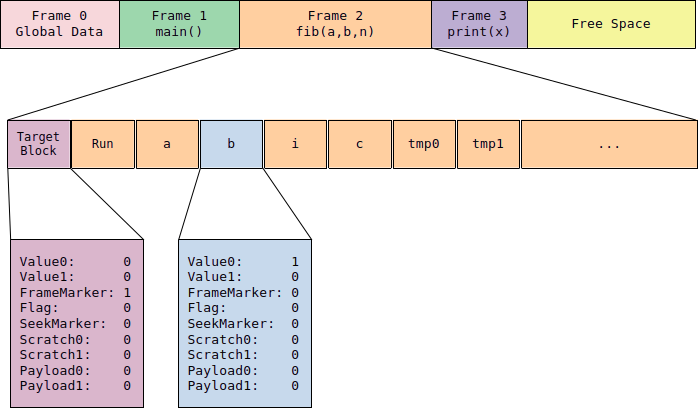
\includegraphics[width=0.8\textwidth]{img/tape_hierarchy}
  \caption{Acus tape hierarchy: the tape is divided into frames, which are divided into slots, which consist of macro-cells containing 9 fields (BF-cells).}
  \label{fig:tapehierarchy}
\end{figure}

\subsubsection{Cells and Macro-Cells}
A raw BF cell is only directly useful for the eight primitive BF commands. Acus therefore treats groups of raw cells as one logical macro-cell. This subsection should explain the purpose of the value fields, scratch fields, flag field and transport fields at a conceptual level: not as an exhaustive memory-layout specification, but as the reason why higher-level operations can be expressed locally around each logical value.

\paragraph{Suggested figure.}
Show one macro-cell as a horizontal strip of nine BF cells. Label only the conceptual roles: value, scratch, flag, marker and payload. Avoid naming every implementation field if that makes the figure too dense.

\subsubsection{Slots}
A slot is the compiler-visible storage location for one value. Small values may occupy a single macro-cell, while larger values occupy a sequence of macro-cells. This is the right place to explain why slots are more useful than raw addresses: the compiler can reason about copying, clearing, arithmetic and lifetime at the level of values rather than individual BF cells.

\paragraph{Suggested figure.}
Show three slots of different sizes placed consecutively on the tape, for example an 8-bit integer, a 16-bit integer and a small array. This figure should make clear that slot size follows from the represented type.

\subsubsection{Slot Proxies}
Not every expression denotes a fixed slot. Array elements, dereferenced pointers and fields inside aggregate values may be known only indirectly. Acus represents such locations as slot proxies: objects that describe how to reach or construct access to a value without necessarily materializing it immediately. This subsection should introduce the distinction between a direct slot and a delayed access path.

The important point is conceptual: a proxy is a description of a location or computation that can be turned into BF code when needed. This makes it possible to write high-level expressions that look like ordinary reads and writes, while the compiler still decides how much work has to be generated.

\paragraph{Suggested figure.}
Use a small tree diagram: a root slot for an array, an index expression, and a proxy representing the selected element. A second small example could show a pointer slot leading to a dereferenced target.

\subsubsection{Frames}
A frame groups all data belonging to one function activation. Each frame contains the local control cells, optional return storage, arguments, named locals and compiler-generated temporaries. Function calls can then be viewed as transitions between frames: the caller prepares the callee frame, jumps to the callee's entry block, and later resumes execution using the return information stored on the tape.

This subsection should stay at the model level. The goal is to show that Acus simulates a call stack on top of the BF tape, not to document the precise constructor code used to allocate or release frame data.

\paragraph{Suggested figure.}
Show a call stack with a global frame, a caller frame and a callee frame. Highlight the current frame and indicate where arguments, return slot and local variables live.

\subsection{Code Generation Patterns}
This section should introduce the small set of BF idioms from which larger operations are assembled. It should not become a catalogue of every algorithm in the compiler. Instead, it should show enough examples to make the generated code feel less magical.

\subsubsection{Clearing, Moving and Copying Values}
The simplest useful BF idiom is destructive movement: consume one cell while adding its value somewhere else. From that, one can build clearing, moving and non-destructive copying by introducing temporary storage. These operations are worth including because they appear everywhere: assignments, argument passing, return values and arithmetic all rely on them.

\paragraph{Suggested figure.}
Use a before/after tape diagram showing a destructive move from cell \(A\) to cell \(B\), followed by a non-destructive copy using a temporary cell. This can be shown without writing the full BF sequence.

\subsubsection{Addition and Subtraction}
Addition and subtraction are the natural next step after copying. For small values, they are implemented by transferring counts between cells; for multi-cell values, the algorithm has to propagate borrow or carry between macro-cells. This subsection should explain why arithmetic on a BF tape is not a single operation but a choreography of local loops.

Include addition and subtraction as the main arithmetic examples. They are fundamental enough to justify space, while multiplication and division can be mentioned only briefly as repeated or derived algorithms unless they become important in a later case study.

\paragraph{Suggested figure.}
A two-row diagram works well here: the first row shows single-cell addition, the second row shows multi-cell addition with a carry flag moving to the next macro-cell.

\subsubsection{Comparison and Boolean Results}
Conditionals and loops require values to be converted into flags. The most useful comparisons to feature are zero/nonzero, equality and less-than. These are enough to explain how high-level control flow becomes BF block selection: the comparison produces a boolean value, and that value is then used to choose the next target block.

This subsection should emphasize the output of comparison algorithms rather than every internal step. The reader should come away understanding that comparisons are compiled into ordinary tape transformations whose result is stored in a normal slot or flag cell.

\paragraph{Suggested figure.}
Show an expression such as \texttt{i < n} being lowered into a temporary boolean slot, followed by a block-selection decision. This connects the arithmetic section back to the program-structure section.

\subsubsection{Selected Algorithms to Omit or Defer}
Do not spend chapter space on every operation Acus can generate. Multiplication, division, modulo, string formatting and input parsing can be summarized in a short paragraph or deferred to examples if needed. The chapter will be stronger if it focuses on the operations that reveal the underlying model: move/copy, add/subtract, compare and dynamic pointer movement.

\subsection{Pointer Movement}
BF has no random access instruction; the only way to reach a cell is to move the pointer step by step. This makes pointer movement one of the central code-generation problems in Acus. The compiler must constantly choose between generating a known relative move and generating a runtime search or traversal.

\subsubsection{Static Pointer Movement}
When the source and destination locations are known at compile time, pointer movement is straightforward: emit the required number of \texttt{<} or \texttt{>} commands. This is the common case for local slot operations within a frame. The compiler can keep track of the current pointer position and avoid unnecessary moves by scheduling nearby operations together where possible.

\paragraph{Suggested figure.}
Show a tape with a current pointer position and a target slot at a known offset. Annotate the resulting BF movement as a fixed sequence of arrows.

\subsubsection{Frame-Relative Movement}
Most ordinary local variables can be addressed relative to the current frame. This subsection should explain the role of frame markers and known frame layouts: even though the underlying BF tape is flat, Acus imposes structure on it so that generated code can move predictably within the active frame.

This is a good place to connect the frame abstraction to the cost of generated code. A variable that is close to the current pointer is cheap to access; one that is far away requires a longer sequence of moves. The layout of frames and temporaries therefore directly influences the generated BF size.

\paragraph{Suggested figure.}
Show the same function frame twice: once as an abstract frame with named slots, and once as a linear tape with offsets from the frame marker.

\subsubsection{Dynamic Pointer Movement}
The most interesting pointer-movement algorithms are the ones where the target is not known until runtime. Examples include array access by a computed index, pointer dereferencing and moving data to a slot selected by a runtime value. These algorithms rely on metadata stored in macro-cells: markers, counters and payload fields are used so that the BF pointer can search through structured tape data and stop at the correct logical cell.

This is the pointer-movement algorithm most worth featuring in detail. It captures the central difficulty of compiling to BF: the target address is not available as an address, so it must be represented as data on the tape and consumed by a traversal algorithm.

\paragraph{Suggested figure.}
Show an array slot with several elements and an index value stored elsewhere. Then show a runtime traversal in which the index is decremented while the pointer advances from element to element until the selected element is reached.

\subsubsection{Payload Transport}
Dynamic writes are harder than dynamic reads because data has to be carried to a location that is not statically known. Acus solves this by moving values through designated payload fields. The payload travels along with the dynamic traversal and is deposited when the target macro-cell is found.

This subsection should describe the idea at a high level, because it is one of the more distinctive algorithms in the compiler. It also gives a natural explanation for why macro-cells contain more than just value storage.

\paragraph{Suggested figure.}
Use a three-stage diagram: prepare payload, traverse to dynamic target, commit payload into the selected value field.

\subsection{Control Flow and Functions}
This section should tie the earlier pieces together: arithmetic produces flags, flags select blocks, blocks update the target-block cell, and function calls are represented as jumps between frames.

\subsubsection{Conditionals}
An \texttt{if}-statement becomes a small control-flow graph. First, the condition expression is evaluated into a temporary boolean slot. Then the current block selects one of two successor blocks. Both branches eventually continue at a join block, unless they return or jump elsewhere.

\paragraph{Suggested figure.}
A minimal control-flow graph for \texttt{if/else}: condition block, then block, else block and join block. This should visually resemble Figure~\ref{fig:fibflow}.

\subsubsection{Loops}
A high-level loop is compiled as a cycle in the block graph. The condition block either jumps into the body or exits to the block after the loop. The body eventually jumps back to the condition block. \texttt{break} and \texttt{continue} are then just additional edges in this graph.

\paragraph{Suggested figure.}
Show a loop as four blocks: preheader, condition, body and exit. Add dashed arrows for \texttt{break} and \texttt{continue}.

\subsubsection{Function Calls and Returns}
A function call consists of preparing the callee frame, copying arguments into it, storing enough return information to resume the caller, and selecting the callee's entry block. Returning reverses this process: the return value is written to the caller's expected location, the caller frame becomes active again, and the target block is set to the continuation block.

Keep this subsection conceptual. The aim is to explain that calls and returns are not BF primitives but conventions implemented on the tape and in the block scheduler.

\paragraph{Suggested figure.}
A timeline figure would be useful: caller before call, callee active, caller after return. Indicate how the active frame changes and where the return value goes.

\subsection{Caching and Materialization}
\label{sec:compiling:cache}
The caching system is the one implementation-oriented topic worth treating in more depth, because it explains how Acus avoids generating an excessive amount of BF for repeated accesses to the same logical values. Without caching, every read and write would immediately synchronize all relevant tape locations, leading to large and slow programs.

\subsubsection{The Problem: Repeated Materialization}
Slot proxies allow expressions to remain abstract until their value is needed. However, repeatedly materializing the same proxy can duplicate work. For example, accessing the same array element or struct field several times in a block should not require recomputing the entire access path each time.

This subsection should present the problem using a simple expression such as \texttt{x = a[i] + a[i]}. The compiler should recognize that both occurrences refer to the same logical location, while still being conservative when aliases or writes might invalidate that assumption.

\paragraph{Suggested figure.}
Show two identical proxy trees leading to the same materialized slot. Then show the optimized version where the first materialization is reused.

\subsubsection{Cache Entries}
A cache entry connects a logical proxy to a concrete slot that currently holds its materialized value. The cache is therefore not merely a value cache; it is a bridge between abstract access paths and physical tape storage. Entries can be clean, dirty or invalid depending on whether the concrete slot agrees with the underlying logical location.

This subsection may include a little more detail than the rest of the chapter, but it should still be written in terms of invariants rather than C++ classes. The key invariant is that generated BF must observe the same values as if every proxy access were performed directly.

\paragraph{Suggested figure.}
Use a table-like figure with columns \emph{proxy}, \emph{materialized slot}, \emph{state} and \emph{meaning}. Keep it small: three or four entries are enough.

\subsubsection{Reads, Writes and Dirty State}
Reads may reuse a clean cache entry. Writes are more subtle: writing through one proxy may invalidate cached values for the same location or for locations below it in the proxy tree. A write can also make a materialized slot dirty, meaning that its value must eventually be committed back to the underlying location.

This is the place to explain parent/child invalidation at a conceptual level. For example, writing to an array element should invalidate cached views of that element and possibly cached views of the containing array, depending on what assumptions the cache had made.

\paragraph{Suggested figure.}
Show a proxy tree for an aggregate value. Highlight the subtree invalidated by writing to one child element.

\subsubsection{Boundaries}
The cache is allowed to be clever only where control flow and aliasing are under control. At function calls, jumps and other control boundaries, Acus conservatively flushes or invalidates cached state. This mirrors the role of synchronization in the Synapse-191 hardware: values may temporarily live in a faster or more convenient representation, but they must be made consistent before the next part of the program relies on them.

A useful comparison can be made here to the A and V flags from the hardware chapter. Synapse-191 tracks whether the data pointer or data value has changed so it can avoid unnecessary RAM traffic; Acus generalizes this idea from one hardware register to many compiler-managed tape locations.

\paragraph{Suggested figure.}
Show a block with several cached operations internally, followed by a control boundary where dirty entries are flushed and uncertain entries are invalidated.

\subsubsection{Aliasing and Conservative Choices}
The hardest cache cases arise when two different proxies might refer to the same storage, such as through pointers or dynamic array indices. Acus should prefer correctness over cleverness here. When a write may be visible through another access path, the cache must assume that related entries are no longer trustworthy.

This subsection should be honest about the trade-off: conservative invalidation can generate more BF, but it prevents subtle wrong-code bugs. This is also a good place to mention that pointer writes are deliberately treated as immediate visibility boundaries.

\paragraph{Suggested figure.}
Show two different access paths converging on the same slot: one through a named variable, one through a pointer. Mark the cache entries that become invalid after the pointer write.

\subsection{Selected Case Studies}
Rather than listing every supported language feature, this section should use a few examples to show how the previous ideas combine. Each case study should be short and should include either generated BF statistics, a tape diagram, or a control-flow diagram.

\subsubsection{A Small Arithmetic Example}
Use a compact program that computes a value using assignment, addition, subtraction and comparison. The goal is to connect slots, temporaries, arithmetic idioms and block selection in one example.

\paragraph{Suggested figure.}
A side-by-side view: high-level pseudocode on the left, simplified block graph or tape effects on the right.

\subsubsection{Dynamic Array Access}
This is the best pointer-movement case study. An expression like \texttt{arr[i] = arr[i] + 1} involves dynamic reads, arithmetic and a dynamic write. It also stresses caching: the two appearances of \texttt{arr[i]} may be related, but the write must still be handled carefully.

\paragraph{Suggested figure.}
A sequence diagram showing materialize \texttt{arr[i]}, increment temporary, write back through dynamic traversal.

\subsubsection{Recursive Fibonacci}
The Fibonacci example already introduced block scheduling and frames, so it can be revisited here as a larger integration test. It demonstrates calls, returns, temporaries, conditionals and repeated frame creation. The section should focus on what the generated BF has to simulate, not on the C++ interface used to describe the program.

\paragraph{Suggested figure.}
Show a shallow recursion tree next to a stack-frame diagram. This makes the cost of recursion on a BF tape concrete.

\subsection{Limitations and Trade-Offs}
This chapter should end by making clear that Acus does not make BF efficient in an absolute sense. It makes BF compilation systematic. The generated programs are large because every high-level operation must eventually become pointer moves, cell updates and loops. The value of the compiler is that it makes these transformations reliable and composable.

\subsubsection{Code Size Versus Runtime Work}
Some transformations reduce runtime work but increase program size, while others keep the generated BF short at the cost of more movement at runtime. Caching, temporary reuse and block layout all live in this trade-off space.

\subsubsection{Abstraction Versus Control}
The abstractions used by Acus make it possible to generate BF from structured programs, but each abstraction hides a cost. Frames, slots, proxies and caches are useful precisely because they make those costs manageable rather than invisible.

\subsubsection{Future Directions}
Close with a brief list of possible improvements: better block ordering, more precise alias analysis, more aggressive cache retention across safe boundaries, improved temporary allocation and more specialized arithmetic kernels. This should read as a natural continuation of the techniques in the chapter, not as a new implementation roadmap.
